\PassOptionsToPackage{quiet}{fontspec}
\documentclass{article}
\usepackage[UTF8]{ctex}
% Language setting
% Replace `english' with e.g. `spanish' to change the document language
\usepackage[english]{babel}

% Set page size and margins
% Replace `letterpaper' with`a4paper' for UK/EU standard size
\usepackage[letterpaper,top=2cm,bottom=2cm,left=3cm,right=3cm,marginparwidth=1.75cm]{geometry}

% Useful packages
\usepackage{amsmath}
\usepackage{graphicx}
\usepackage[colorlinks=true, allcolors=black]{hyperref}
\usepackage{amssymb}
\usepackage{titletoc}
\usepackage{titlesec}
\usepackage{fontspec}
\setmainfont{Times New Roman}
\usepackage{subfigure}
\usepackage{tikz}
\usetikzlibrary{positioning,petri}
\usetikzlibrary{arrows.meta,arrows,shapes,automata,backgrounds,petri,patterns,decorations.pathmorphing,positioning,calc,shapes.geometric}%插件
\usepackage{xcolor}
\usepackage{tcolorbox}
\usepackage{algorithmic}
\usepackage{diagbox}
\usepackage[ruled,vlined,linesnumbered]{algorithm2e}
\usepackage{tabu}
\usepackage{multirow}
\usepackage{booktabs}
\usepackage{framed}
\usepackage{hyperref}

\RequirePackage{xeCJK} 
\setCJKfamilyfont{KaiTi}{KaiTi} \newcommand{\song}{\CJKfamily{KaiTi}}


\hypersetup{
    colorlinks=true,
    linkcolor=black,
    filecolor=magenta,      
    urlcolor=blue,
    pdftitle={Overleaf Example},
    pdfpagemode=FullScreen,
    }







\titleformat{\section}{\normalfont\Large\bfseries}{\thesection.}{0.2em}{}
\titleformat{\subsection}{\normalfont\large\bfseries}{\thesubsection}{0.2em}{}

\newtheorem{definition}{Definition}
\newtheorem{example}{Example}
\newtheorem{problem}{Problem}
\newtheorem{remark}{Remark}
\newtheorem{derivation}{Derivation}
\newtheorem{proposition}{Proposition}




\begin{document}




\title{
\includegraphics[width=1.2in]{MUST.png}\\[-2pt]\huge Macau University of Science and Technology
	~\\
	Faculty of Innovation Engineering
	~\\
	Dept. of Engineering Science
	~\\
	\LARGE{(澳門科技大學創新工程學院工程科學系)}
	~\\[40pt]

	Thesis Proposal
	~\\
	(論文選題報告)
	~\\[40pt]

	\textbf{\LARGE Research on the Structure of Offline Handwritten Signature Verification Models Based on Transformer}

	\title{}

	~\\[50pt]





	\large{

		Submitted by: Mingchen Wang


		~\\[1pt]

		Student No.: 2230025907

		~\\[1pt]

		Supervisor: Xin Liu}

}

\author{}

\date{}


\titlecontents{section}[0pt]{\addvspace{5pt}\filright}
{\contentspush{\thecontentslabel\
	}}
{}{\titlerule*[8pt]{.}\contentspage}


\maketitle
\thispagestyle{empty}

\clearpage




\pagenumbering{roman}
\renewcommand{\abstractname}{\Large Abstract\\}
\begin{abstract}
	Offline handwritten signature verification is a specific application of biometrics technology, based on a handwritten signature provided by an individual to verify his/her identity. It is routinely used in security authentication, financial transactions, access control systems and other security areas. 

    Offline handwritten signature verification consists of two types of tasks: author-dependent and author-independent. The first task is to verify a handwritten signature against a database of user handwritten signatures. The second task is to determine whether a signature is forged or not by using only the provided handwritten signature.

	The research content of this paper includes: 1. studying and reproducing the model architecture of fusion of Convolutional Neural Network and Transformer to realize the model architecture of combining local and global features of learning images. 2. propose an end-to-end offline handwritten signature verification model architecture OSVTF that combines Convolutional Neural Networks and Transformer to extract handwritten signature image features in a more comprehensive way. 3. First use Support Vector Machines as feature classifiers to identify whether a handwritten signature is fake or not, and then give better feature classifiers based on the research results to realize the offline handwritten signature verification model architecture with better performance.

	\textbf{keywords}: Offline handwritten signature verification; end-to-end; Transformer; OSVTF; support vector machine.
\end{abstract}

\phantomsection\addcontentsline{toc}{section}{Abstract}\tolerance=500



\newpage


\clearpage

\renewcommand{\abstractname}{\Large 摘要\\}
\begin{abstract}
	\medskip
	離線手寫簽名驗證是生物特徵技術的一個具體應用, 基於個人提供的手寫簽名以驗證身份. 日常用於安全認證, 金融交易, 存取控制系統和其他安全領域. 

    離線手寫簽名驗證包含兩種類型的任務: 作者依賴和作者獨立. 第一種任務是將手寫簽名與資料庫的對應用戶手寫簽名進行對比驗證。第二種任務是僅透過提供的手寫簽名來判斷簽名是否偽造

	本文研究内容包括: 1, 研究與復現卷積神經網絡與Transformer融合的模型架構,以實現結合學習圖像局部特徵和全局特徵的模型架構. 2. 提出端到端的一種結合卷積神經網絡和Transformer的離綫手寫簽名驗證模型架構OSVTF,能夠更佳全面地提取手寫簽名圖像特徵. 3. 先使用支持向量機作爲特徵分類器以鑒別手寫簽名是否為僞造的,根據調研結果給出更優秀的特徵分類器,實現更優秀性能的離綫手寫簽名驗證模型架構。

	\medskip
	\textbf{關鍵詞}:離線手寫簽名驗證; 端到端; Transformer; OSVTF; 支持向量機.
\end{abstract}

\phantomsection\addcontentsline{toc}{section}{摘要}\tolerance=500

\newpage



\ctexset{ contentsname = {Table of Contents}}

\tableofcontents

\phantomsection\addcontentsline{toc}{section}{Table of Contents}\tolerance=500
\newpage

\pagenumbering{arabic}
\setcounter{page}{1}

\section{Introduction}
\subsection{Research Background}

Biometrics technology is a technology that identifies or verifies individuals based on their physiological characteristics such as features, face, iris, or behavioral characteristics such as voiceprints and handwritten signatures. The technology is widely used in security fields such as security authentication in enterprises, financial transactions, access control systems, etc \cite{1}.

This technology is mainly used in identification and verification scenarios. In the first scenario, users only need to provide samples of their individual or physiological characteristics, and the biometric system identifies the user who provides the characteristics among the registered users based on the samples. The second scenario, on the other hand, is based on the first scenario, where one declares one's identity to the system, and then the system will verify whether any of the registered users is a designated user based on the above information.

Handwritten signature is a more important individual behavioral feature in daily life because it serves as the main feature for verifying personal identity in legal, financial, and administrative fields. Also because it cannot be invaded during the collection process, handwritten signatures are considered as one of the main features in many techniques for verifying personal identity. This leads to the specific application of handwritten signature verification, where the identity of a statement is authenticated based on the comparison of the signature provided by the user (defined as a Query) with the signature stored by that user in the system (defined as a Reference).

Based on the above, handwritten signature verification belongs to a specific application of biometric verification scenarios, which will be categorized into offline and online according to different collection routes. Offline Handwritten Verification has a personal signature collection process that is obtained through the user's writing process on paper, while Online Handwritten Verification uses a digitizing station to collect the user's handwritten signature features, and thus The collected handwritten signature image may be affected by the device such as pen position, tilt, pressure etc. This shows the advantages of offline handwritten signatures, which can be used to collect an image of a user's personal signature anytime, anywhere and without device limitations to authenticate an individual's identity.

The study of offline handwritten signature verification will provide a more comprehensive understanding and comparison of the difference between traditional machine learning methods in the past and deep learning methods in the last decade for offline handwritten signature verification, so as to propose a handwritten signature verification model architecture with more efficient and accurate. As a result, the security field can be replaced by a more secure handwritten signature verification model or algorithm that can more efficiently and accurately complete each user's personal identity verification request, thus saving the time cost of machine verification, providing more computer reasoning resources and planning time for other core tasks, and to a certain extent saving the cost of verifying personal identity. As the new model architecture is proposed, it will provide a new design or improvement scheme to the existing model, thus deriving more excellent offline handwritten signature verification model architecture, thus advancing the research level of offline handwritten signature verification model or algorithm.

\subsection{Motivation}

Although offline handwritten signature verification will not be affected by factors such as digitizers during data collection, it is not possible to guarantee that the signatures obtained multiple times will be exactly the same when users write their personal signatures on paper. It may also be affected by physical pens, paper thickness, etc. Therefore, the preprocessing process after data collection will affect the system verification effect to a certain extent. A good image preprocessing technique will directly affect the system verification performance.

In the past research on offline handwritten signature verification, scholars have taken traditional machine learning methods based on sample distribution in order to design image features to verify whether the signature is forged or not \cite{1}. However, this method has defects, the verification credibility and accuracy rely heavily on manually designed features, and there are restrictions on the font style of handwritten signatures and other requirements, and the time cost of data preprocessing is very huge. With the development of deep learning and convolutional neural network, in recent years, scholars gradually take the convolutional part of the convolutional neural network to reason about handwritten signatures, and the multi-channel feature map obtained from the reasoning is used as the feature vector of handwritten signature verification. This supervised learning feature extraction method has achieved good results \cite{2}. However, the multi-channel feature maps extracted only by convolutional neural network will cause the process of learning image features to be missing some global features because of the shared parameter convolution kernel operation of the convolutional layer in its model architecture. Based on this, scholars have proposed a Vision Transformer architecture \cite{10} with better performance based on Transformer \cite{9} for image classification tasks. Compared with convolutional neural network, experiments have shown that the attention mechanism inside Transformer has better global feature learning ability, which can accumulate the attention weights in the important parts of the features and pay more attention to the effective features. It is expected to propose an architecture that can make up for the lack of global feature learning ability of convolutional neural networks (CNN), so as to better combine the excellent local feature learning ability of convolutional neural networks.

Offline handwritten signature verification consists of two tasks: Writer-Dependent (WD) and Writer-Independent (WI). the WD task requires Reference and Query to verify the handwritten signature samples to verify whether the signatures are forged or not, and to a certain extent, it depends on the features of the writer's Reference. the WI task requires only the Query to verify the signature samples, and to a certain extent, it relies on the features of the writer's Reference. WI task is to verify whether the signature is forged by Query only, and will not depend on the Reference feature of the writer. In the past, scholars adopted Support Vector Machines as feature classifiers to verify whether a handwritten signature is forged or not based on manually designed features. When the image size is larger, the number of features is more, which leads to the model parameters of the support vector machine are difficult to converge, increasing the overall model architecture training cost. Thus, it is expected to propose a feature classifier that can converge faster and outperform the support vector machine.



\subsection{Research Objectives}

For the WD and WI tasks, the main objectives of this paper are as follows: 1. to reproduce the OSV (Offline Signature Verification) model; 2. to propose an OSV model architecture that combines the local feature learning capability of convolutional neural networks and the global feature learning capability of Transformer; 3. to propose faster convergence and better results of support vector machines for offline handwritten signature feature classifier

In the first stage, the existing newer OSV models are reproduced to analyze and summarize the details and features of the OSV model architectures, and to find out the commonalities and shortcomings among them, so as to better find the key points and methods for optimization.

In the second stage, a Transformer-based optimization scheme is proposed on the basis of the reproduced model, and comparison experiments are taken to verify that the model performance is better than the previous model performance. During the comparison experiments, the image preprocessing and validation methods are constrained to be consistent, so as to find out the final training and validation scheme suitable for the model architecture.

In the third phase, since the convolutional neural network in the image classification task is different from the offline handwritten signature verification task in terms of final output category probability, the support vector machine is used on the proposed model to experiment whether the extracted image features can be used effectively, and then replaced by a feature classifier with better results.


\newpage
\section{Literature Review}

Biometrics technology is widely used in various security applications. The purpose of such systems is to identify a person based on physiological or behavioral characteristics \cite{1}. This technology recognizes a person by fingerprints, face, iris and other information in addition to the handwritten signature of the individual to identify the individual.

Handwritten signatures can be used for both identification and verification tasks. The handwritten signature recognition task is given a handwritten signature of a person and the system will look for the user in the database who matches this handwritten signature based on this signature. The handwritten signature verification task is that the user provides a handwritten signature while declaring to the system that he or she is a certain user in the database, and then the system compares his or her handwritten signature with the corresponding database of handwritten signatures of users in the database, thereby verifying whether or not he or she is indeed such a person.

The handwritten signature verification task is classified into two types based on the data: offline and online.Offline means that the signature of a different person is captured on a piece of paper by the individual and then scanned for verification.Online means that the signature is recognized by the digitized tablet from which the individual has signed \cite{3}. The former approach is not affected by the digitizing tablet model, so offline handwritten signature verification does not require much manipulation in the data preprocessing process to obtain a purely personal written signature.

Regardless of offline or online handwritten signatures, the data they collect are image data, so a good data preprocessing technique will surely improve the system verification accuracy. In order to improve the quality of signature images, scholars have adopted the conversion of RGB images to GRAY single-channel images, and some even use pixel-smoothing image processing in order to remove noise \cite{4}.

Early offline handwritten signatures are adopted machine learning approach, such as Edson et al. proposed an offline signature verification system using Hidden Markov Model \cite{5}. This traditional machine learning approach is flawed: this method is extremely dependent on manually designed features for training, and the accuracy of classification is directly related to these features \cite{2}. With the development of deep learning and convolutional neural networks, in 2012 Krizhevsky A. et al. proposed AlexNet \cite{6} to win the ImageNet competition on the task of image categorization well ahead of the second participant who used a traditional algorithm. This made deep learning represented by convolutional neural networks gradually become the mainstream of image tasks, and academics subsequently introduced deeper convolutional neural networks such as VGG \cite{7} and ResNet \cite{8} with residual connectivity. These convolutional neural networks are composed of multiple convolutional layers and linear layers, and the front part of the convolutional layer uses a convolutional kernel with shared parameters to traverse the values of image pixels, so as to achieve the effect of learning image features. The difference between the image features extracted in this way and the traditional image feature extraction methods is that the way of feature extraction by convolutional neural network is supervised learning, which must rely on the amount of data to have a better feature extraction effect. As a result, convolutional neural networks have an inherent advantage in the image classification task, even though the final classification still outputs the category probabilities through the prior layer.

The above mentioned convolutional neural network uses a convolutional kernel to traverse the image pixels in order to learn the image features, but the convolutional operation suffers from the defect of local field of view. Although it is able to learn local features of an image, it is less effective in learning global features, resulting in the image classification task of convolutional neural networks in the more excellent recognition accuracy there is an obstacle to achieve the best recognition accuracy. With the development of deep learning in the field of natural language processing, in 2017 Vaswani A. et al. proposed the Transformer model for machine translation \cite{9}. The model adopts the Encoder-Decoder mainstream structure for machine translation, and unlike previous deep learning models for machine translation, Transformer introduces an attention mechanism. Under the effect of the attention mechanism, it is able to perform global feature perception on word vectors, and refer to the feature information of the previous word and the feature information of the input word vectors when generating the predicted words, so it can generate sentence predictions of different lengths. Moreover, experiments have proved that Transformer has better global generalization ability than previous Encoder-Decoder machine translation models.

In view of Transformer's ability of attentive global feature perception, Dosovitskiy A. et al. firstly used Transformer Encoder for image categorization task in 2021, named Vision Transformer (ViT) \cite{10}.The internal structure of ViT completely discards the convolutional layer, and takes the input images as a whole. The internal structure of ViT completely abandons the convolutional layer and takes the input image as a patch and Embeddings operation, the embedding of each patch is treated as a single token of word vectors, and then the image is flattened and entered into the Transformer Encoder as word vectors, which is passed through a number of Encoder Layers, and then a MLP is set up to map category probabilities in order to complete the image categorization task. The task of image categorization is accomplished. Experiments have shown that this way of modeling has obtained recognition accuracy ahead of convolutional neural networks in image classification tasks, which has also led to the derivation of CNN + Transformer deep learning model structures, such as DETR for image target detection \cite{11} and MaskFormer for image segmentation \cite{12}. This approach takes a Linear layer convolutional neural network that removes the final classification, inputs the image to extract multi-channel features, and uses the features as input vectors for the Transformer to perform global feature sensing.DETR, the pioneering work of CNN + Transformer, is validated in MS COCO \cite{13}, although not as well as previous R-CNN \cite{14}, which adopts post-processing operations such as NMS. R-CNN, YOLO series network \cite{15}, the recognition accuracy is high, but the advantage of this approach is that it does not need any pre-setting of target detection a priori boxes such as Archer Box and NMS post-processing, which is an end-to-end model structure. This approach simplifies the model inference process to a certain extent, but it also increases the cost of model training time, and requires the design of a finer training scheme to ensure the convergence of model parameters.

Transformer has excellent global feature perception capability compared to CNN on image tasks, so scholars in the field of offline handwritten signature verification have proposed a Transformer-based model architecture TransOSV \cite{16}. The model adopts similar Encoder-Decoder architecture, the input Reference and Query are pre-processed by RGB to GRAY image, and then enter into the ViT Encoder as Holistic Encoder, then the output of Holistic Encoder is subjected to convolution operation, and finally the features of Reference and Query are subjected to Contrastive Encoder. and Query features for Contrast based Part Decoder operation. In the training process, TransOSV aggregates the output class features of the Transformer Encoder, the output features of the convolution module, and the output features of the decoder to compute the training loss to complete the model training, and finally the feature classifiers also adopt the Support Vector Machine to verify whether the signature is forged or not. The architecture in Decoder's Cross-attention will Reference features and Query features for attention calculation, the Reference and Query features for the relevance of attention learning, can be better linked to the relationship between Reference and Query. But this architecture will lack the image multi-channel feature information to some extent due to the fact that the input image is directly patched and Embeddings into the Transformer Encoder. Since the image size of ViT is globally constrained, some key information will be lost when the image is resized.

To summarize, in this paper, based on the TransOSV [16] architecture, we will adopt the CNN + Transformer approach, where the multichannel feature maps are extracted by the CNN before the image enters the Transformer Encoder, and then enter the Transformer to complement the global feature information. In addition the Holistic Encoder architecture is optimized to be able to accept image size variations, thus better adapting to the experimental scenarios with different dataset samples.



\newpage
\section{Offline Signature Verification TransFormer}

In this section, the methods used are first summarized and the proposed model structure is described in detail. The specific details of the proposed feature extractor containing encoder, convolution module, and decoder structures are analyzed in depth. This will be followed by the details of the loss function, optimizer, and writer-independent classifier \cite{17} for the model parameter training process. Finally, experiments on whether or not to share the model parameters of the feature extractor, and the types of classifiers will be described to achieve good results for the offline verification task of handwritten signatures.

\begin{figure}[htbp]
	\centering
	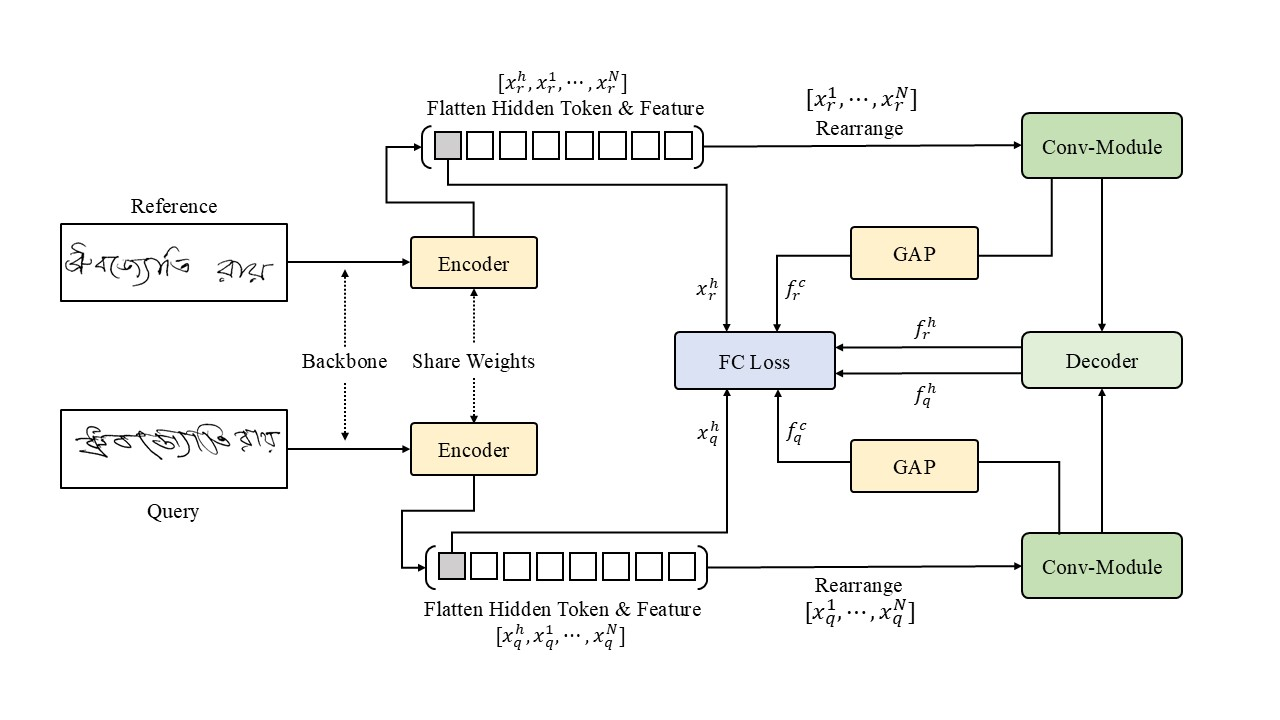
\includegraphics[scale=0.45]{figure/p1.jpg}
	\caption{Offline Signature Verification TransFormer (OSVTF)}\label{fig:p1}
\end{figure}

\subsection{Overview}

The proposed OSVTF is shown in Fig. \ref{fig:p1}. A pair of handwritten signature images Reference and Query of the same size are input. the first passes through the Backbone to extract the multichannel feature map. Then the multi-channel feature maps are passed through a weight-sharing Encoder to learn the image features, and this part of the inference will extract a pair of flat feature tokens $x_r^h,x_q^h$ and a pair of flat feature maps $[x_r^1,\cdots,x_r^N]$. Subsequently the flat feature maps will be reshape to 2D image vectors before inference by convolution module. The output of the convolution module will be divided into two directions: the first direction will pass through the Global Average Pooling layer to get the flat convolutional features $f_r^c,f_q^c$; and the other direction will pair into the Decoder to get the flat attentional decoding features $f_r^h,f_q^h$. The training process will collect the flat feature tokens $x_r^h,x_q^h$ in the inference process, and the training process will collect the flat feature tokens $x_r^h,x_q^h$ in the inference process. $x^h,x_q^h$, flat convolutional features $f_r^c ,f_q^c$ and flat attentional decoding features $f_r^h,f_q^h$ during the inference process will be collected to perform Focal Contrast Loss (FC) loss computation to train the model weights. The Encoder, Decoder and Conv-Module structures are analyzed in depth next.


\subsection{Encoder}

Encoder is following the model structure of ViT (Vision Transformer) \cite{10} shown in Fig. \ref{fig:p2}.

\begin{figure}[htbp]
	\centering
	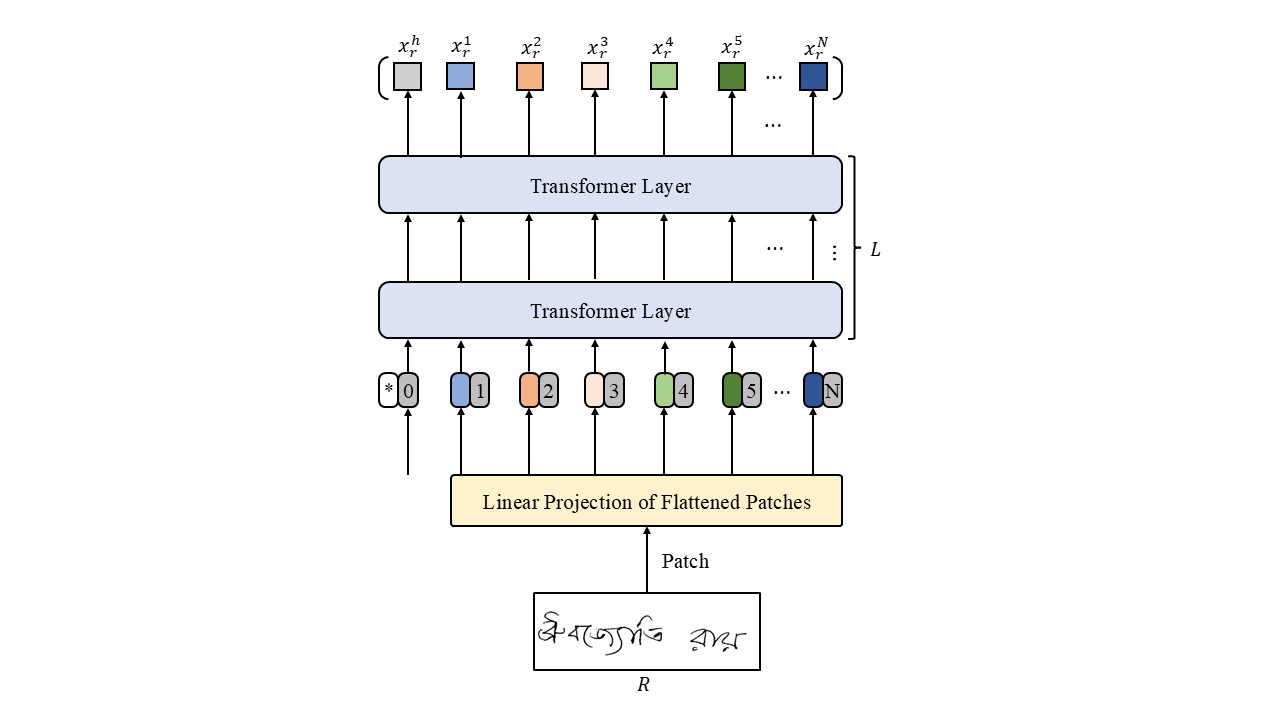
\includegraphics[scale=0.45]{figure/p2.jpg}
	\caption{Vision Transformer structure}\label{fig:p2}
\end{figure}

Take Reference ($C\times H\times W$) as an example, where $C,H,W$ denote the number of image channels, height and width.ViT first divides the input image into N patches and flattens it, where patch number is shown in equation (\ref{e1}).
\begin{equation}\label{e1}
	N = [\frac{(H-P+S)}{S}]*[\frac{(W-P+S)}{S}]
\end{equation}
where $[\cdot]$ denotes the floor function. p and S denote the patch size and the number of convolutional layer steps, respectively, since the original ViT structure takes a convolutional layer in order to accomplish the chunking operation. Next, a learnable weight Class Token and patch image accumulation Position Embedding are spliced in the shape of $(N+1)\times(H\times W)$. Since the Transformer Encoder requires the input to be a Token vector, the relative position information will be lost after the image is patched, so the accumulated Position Embedding reassigns the relative position feature. After the above processing into the L layer Transformer Encoder Layer inference to get the Encoder's flat feature token with feature map $[x_r^h,x_r^1,\cdots,x_r^N ]$,$[x_r^h,x_q^1 ,\cdots,x_q^N]$, the whole Encoder inference as in equation (\ref{e2}).
\begin{equation}\label{e2}
	x_r=[x_r^h,x_r^1,\cdots,x_r^N ]=Encoder([\overline{x}_r^h,E(\overline{x}_r^1),\cdots,E(\overline{x}_r^N )]+pos)
\end{equation}
Where $E(\cdot)$ denotes Embeddings. pos denotes Position Embeddings. each Encoder has the same structure and is formed by $L$ stacks, as shown in Fig. \ref{fig:p3}.

\begin{figure}[htbp]
	\centering
	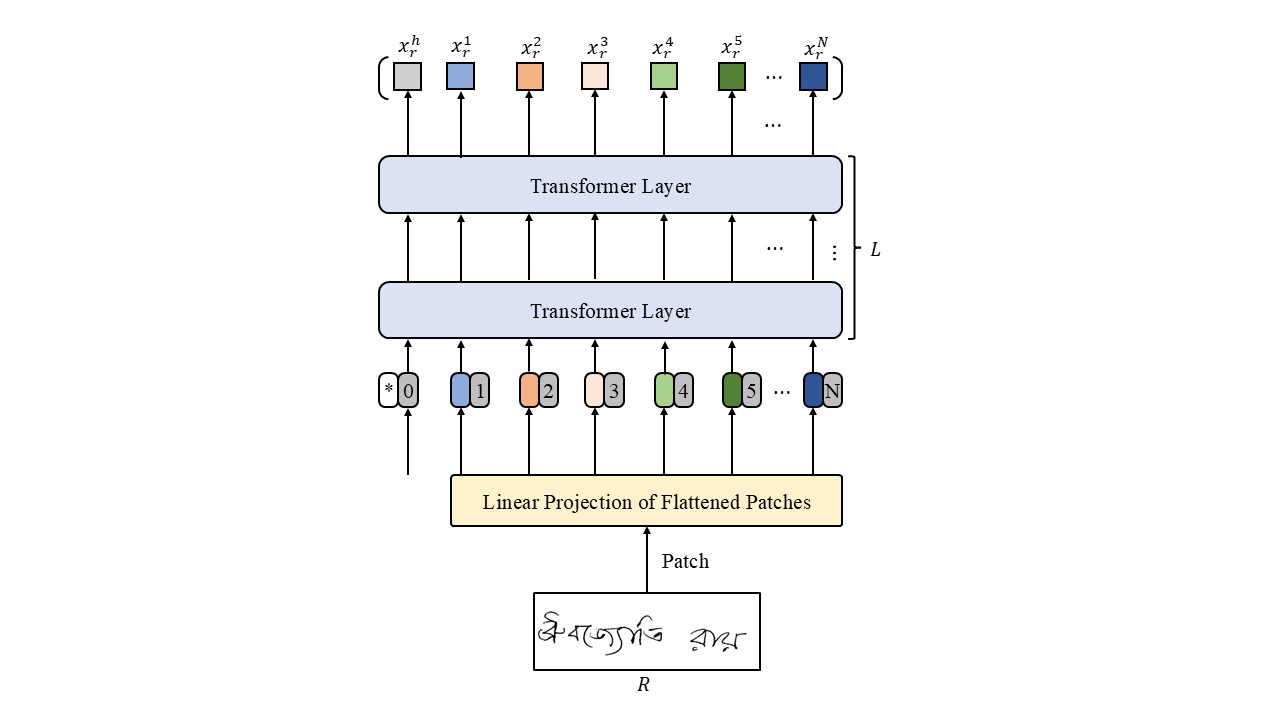
\includegraphics[scale=0.45]{figure/p3.jpg}
	\caption{Multi-Head Attention and Scaled DotProduct Attention}\label{fig:p3}
\end{figure}

Each Encoder Layer consists of a Multi-Head Self Attention (MHSA), Feed Forward Network (FFN), and two Residual Accumulation \& Layer Normalization (LN). First of all, before the input Token enters the Encoder, it will go through three Linear layers to map the input vectors to get $Q,K,V$, and input the mapped three vectors into the MHSA for the attention feature computation.The MHSA in the Encoder is the same as that of the MHSA in the Transformer \cite{9}, which is the same as that of the MHSA of the Transformer, which is the same as that of the MHSA of the Transformer \cite{9}, which is the MHSA of the MHSA of the Transformer. Scaled Dot Product Attention, which is calculated as equation (3).

\begin{equation}\label{e3}
	Attn(Q,K,V)=\mbox{Softmax}(\frac{Q^T K}{\sqrt{d_k }})\cdot V
\end{equation}


where $d_k$ denotes the number of $K,V$ dimensions of the MHSA. Since Scaled Dot Production Attention involves two matrix multiplications of larger size in the computation process, the input process is based on the number of defined heads in order to generate the $d_k$ dimensional linear mapping weights of the number of heads multiplied by 3, which is used to map the input vector into the lower dimensionality of the three matrices $Q,K,V$. At each head, $Attn(Q,K,V ) $operation is performed on each head, and the resulting matrices from the attention computation are finally mapped to the input vector dimensions by a large linear layer. The resulting stacked Transformer Encoder is able to perform the MHSA computation multiple times to better learn the overall vector features.

\subsection{Conv-Module}

The input images are all flattened feature vectors after Encoder, so they need to be reshape to be able to carry out the convolution operation. At the same time, some 2D information will be lost after flattening Token, so the convolution module can make up for some 2D information after reshape. The composition of the convolution module is similar to that of the convolutional neural network, which consists of four Conv2D+ReLUs and two Max Pooling 2Ds in the order shown in Table \ref{tab:t1}.

\begin{table}[htbp]
	\caption{Conv-Module structure information}
	\begin{center}
		\begin{tabu} to 0.8\textwidth{X[2,c]|X[2,c]|X[2,c]}
			%0.8\textwidth   为设置表格宽度  
			%X[c]      表示这一列居中,所占比例为1,相当于X[1,c]  
			%X[3,c]   表示这一列居中,所占比例为3,这列的宽度是X[c]列的3倍  
			\hline
			Layer          & Kernel Size & Output shape              \\
			\hline
			Conv 2D + ReLU & $3\times 3$ & $d_c\times h\times w$     \\
			Conv 2D + ReLU & $3\times 3$ & $d_c\times h\times w$     \\
			Max Pooling 2D & $3\times 3$ & $d_c\times h/2\times w/2$ \\
			Conv 2D + ReLU & $3\times 3$ & $c\times h/2\times w/2$   \\
			Conv 2D + ReLU & $3\times 3$ & $c\times h/2\times w/2$   \\
			Max Pooling 2D & $3\times 3$ & $c\times h/4\times w/4$   \\
			\hline
		\end{tabu}
	\end{center}
	\label{tab:t1}
\end{table}

The output obtained after Conv-Module is propagated in two directions: the first direction is to perform Global Average Pooling (GAP) computation and flattening to obtain the flat convolutional features $f_r^c,f_q^c$; the other direction is to enter the Decoder in pairs for decoding attention computation.

\subsection{Decoder}

\begin{figure}[htbp]
	\centering
	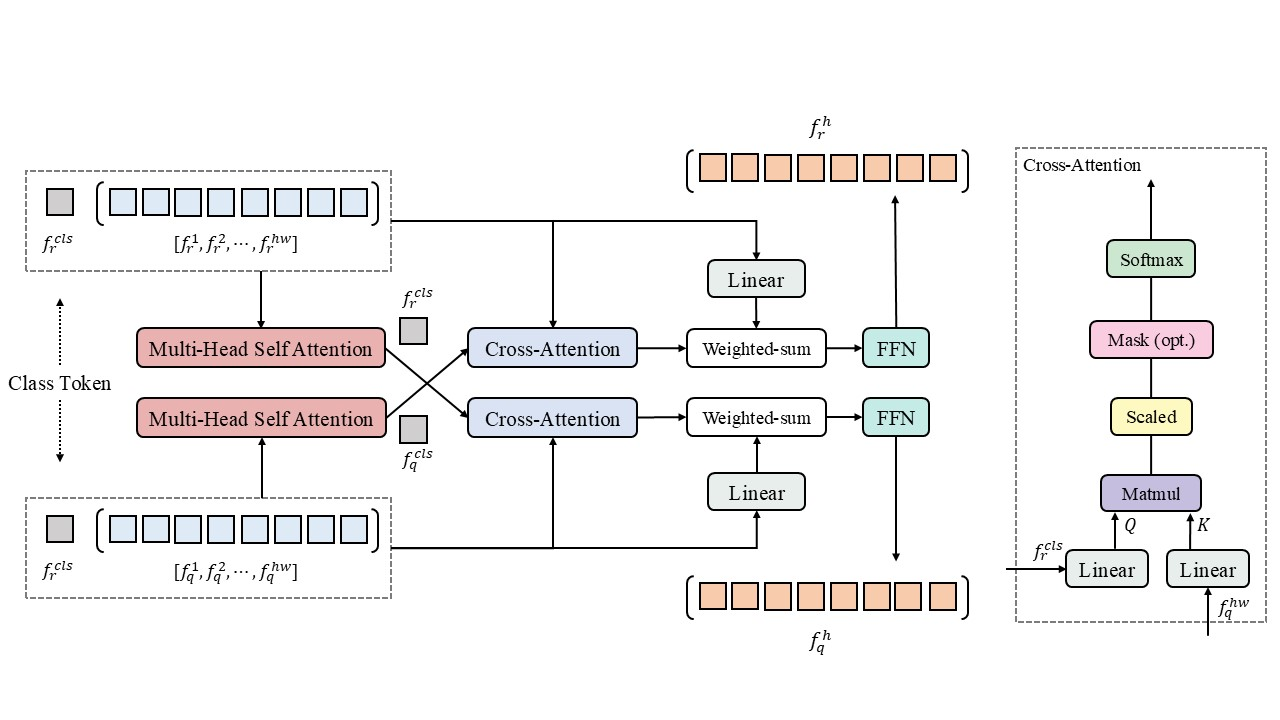
\includegraphics[scale=0.45]{figure/p4.jpg}
	\caption{Decoder and Cross-Attention}\label{fig:p4}
\end{figure}

The Decoder in OSVTF is different from the Transformer Decoder in that it takes two MHSAs and Cross-attention as shown in Figure 4-(a). Similar to the ViT input stage, before inputting the flattened convolutional features, a pair of learnable parameters with the same number of dimensions as the flattened convolutional features, defined as Class Token, is initialized.Its role is the same as that of the Class Token of the ViT-Encoder, which both define an adjusted weight for it to learn whether an image is a forgery or not in a new dimension, thus enabling the model to learn image features better.

Like the above MHSA, the formula is as in Eq. (\ref{e3}).The flat convolutional features inserted with the class token are firstly subjected to MHSA in the Decoder to obtain the flat feature vector of the attention mechanism. Subsequently, in order to be able to learn the relationship between reference and query, Cross-attention is introduced as in Fig. 4-b. Based on the attention mechanism, the linear mapping of $f_r^{cls},f_q^{cls}$ is defined as the Query matrix, and the flattened attention features of the MHSA output are the Key matrix. Similar to MHSA, the attention mechanism is computed based on the learnable parameter class token of reference or query, and in addition the flattened features of the images, to some extent the query matrix inside the attention mechanism can reflect the attention between the images, and since there is no input value Value matrix, Cross-attention gets the attention weights $M_r ,M_q$. This mask weight contains the attention weights of each Token (i.e., each pixel point) between the reference and query, and thus the features of the input Decoder are then accumulated with the attention weights after broadcasting with the Embeddings, and thus what is obtained is a pair of flattened attention features of the attention mechanism. The final Decoder output $f_r^h,f_q^h$ is obtained after FFN, and this pair of features will be subsequently used to optimize the Decoder model parameters according to FC Loss.

\subsection{Loss Function}

The training process of OSVTF will take two loss functions; Sparsity Loss, Focal Contrast Loss.

\subsubsection*{Sparsity Loss}
Since only a few regions in the image of OSV contain discriminative information for signature verification task and $M_r,M_q$ in Decoder has sparsity, the calculation of cross entropy will be taken in order to generate a diverse distribution of contrast-aware masks \cite{16}, so as to better train the linear mapping parameter of Decoder, which is calculated as in Equation (\ref{eq:e4}).

\begin{equation}\label{eq:e4}
	L_{spa}=-\sum_{i=1}^{hw} m_q^i \log(m_q^i ) - \sum_{i=1}^{hw} m_r^i \log(m_r^i)
\end{equation}


\subsubsection*{Focal Contrast Loss}

In previous unsupervised algorithms, comparing the difference between two samples or features was taken to compute the DISTANCE to measure the difference. Define $D(f_r, f_q)$ as the computation of the difference between a pair of flattened feature vectors including the outputs of Encoder, Conv-Module and Decoder. From this, the Contrastive Loss \cite{18} formula for evaluating the difference between two objects can be defined as in equation (\ref{eq:e5}).

\begin{equation}\label{eq:e5}
	L_c = (1 - y) \cdot (D(f_r, f_q))^2 + y \cdot \{\max(m-D(f_r, f_q), 0)\}^2
\end{equation}

where y=1 indicates that the SIGNIFICANCE of the QUERY is FORGED, on the contrary y=0 indicates a forgery. In order to suppress the problem of overfitting in the model training process, double marginal loss is introduced based on CaP \cite{19} as in equation (\ref{eq:e6}).

\begin{equation}\label{eq:e6}
	L_{dm}=(1 - y)\{\max(D(f_r, f_q) - n, 0) \}^2 + y \cdot \{\max(m - D(f_r, f_q), 0)\}^2
\end{equation}

But there is a drawback in the above double marginal loss, when two pairs of REference and query signature samples in which the query is positive, i.e., $y=1$, the distance $d_1,d_2$ of the inference features of the model of two this samples is obtained. If $d_1 >> d_2 > n$, then the loss function should give greater loss/weight to the $d_1$ sample. However, the $d_1, d_2$ samples will be treated equally in the above loss function, so based on the unbalanced training samples case of Focal loss \cite{20}, the final Focal Contrast Loss is improved to get the final Focal Contrast Loss as in Eq. (\ref{eq:e7}).

\begin{equation}\label{eq:e7}
	\begin{aligned}
		L_{fc} & = (1 - y) \cdot \sigma(\overline{K}(D(f_r,f_q) - \alpha_1 )) \cdot \{\max(D(f_r, f_q) - n,0) \}^2 \\
		       & + y \cdot \sigma(\overline{V} (\alpha_2 - D(f_r,f_q )) \cdot \{\max(m - D(f_r, f_q), 0)\}^2
	\end{aligned}
\end{equation}


where $\sigma(\cdot)$ denotes the Sigmoid function. $\alpha_1, \alpha_2$ are the two margin values. $\overline{K}, \overline{V}$ denote the scaling factors.

\subsection{Dataset}

As with the previous public datasets used by scholars, three datasets will be taken to validate the performance of the OSVTF model: the BHSig-B, BHSig-H \cite{21} and CEDAR \cite{22}.

\subsubsection*{BHSig-B \& BHSig-H}

Published by IIT Guwahati. Where BHSig-B is containing handwritten signatures of 100 users in Bengali and BHSig-H is containing 160 users in Hindi. Each user handwritten signature has 24 genuine and 30 forged signatures.

\subsubsection*{CEDAR}

Developed and published by Center of Excellence for Document Analysis and Recognition. The dataset contains 55 users' handwritten signatures in English. Each user signed 24 authentic and 24 forged signatures.

\newpage
\section{Schedule for the thesis}

\subsection*{2024.06 - 2024.10}

Conduct research on OSV models and reproduce OSV model architectures based on CNN and Transformer in recent years. Organize the offline handwritten signature verification public dataset, analyze and summarize the training and inference details of TransOSV model, and complete the reproduction code of TransOSV architecture.

\subsection*{2024.11- 2024.12}

Complete the code to implement the OSVTF architecture proposed in this paper. Investigate academic classifier model architectures or algorithms used for one pair of feature samples, and complete the reproduction code for these classifiers and thus implement them on OSVTF. Develop a model training and validation program for OSVTF and conduct trial runs on GPU servers with the goal of calculating the training model overhead and approximate time to convergence so that the corresponding servers can be leased for model training.

\subsection*{2025.01 - 2025.02}

Conduct the following experiments: 1. Whether the Conv-Module and GAP of OSVTF share parameters. 2. Whether Embeddings in the Decoder of OSVTF share parameters. 3. Whether the Attention operation of OSVTF needs to re-accumulate the positional encoding once. 4. Find out the training hyper-parameters for the best model performance. The first draft will be completed based on the experimental results and feedback from the instructor, and the results will include the proposed first draft and an overview of the latest research progress.

\subsection*{2025.03 - 2025.04}

Revise the thesis based on experimental results and mentor feedback, address issues raised, and prepare to submit the final version of the thesis. Prepare defense materials and presentations.

\subsection*{2024.05 - 2025.06}

Complete final review and formatting of the dissertation and successfully pass the defense, with the final outcome being a master's degree and a published dissertation.

\newpage
\section{Publications}

\begin{itemize}
	\item ``Learning Spatiotemporal Features for Video Semantic Segmentation Using 3D Convolutional Neural Networks,''
	      ISCSIC-2022, IEEE, 14 March 2023, DOI: 10.1109/ISCSIC57216.2022.00023.
	\item ``End-to-End Chinese Lip-Reading Recognition Based on Multi-modal Fusion,'' ICFTIC-2022, IEEE, 27 March 2023, DOI: 10.1109/ICFTIC57696.2022.10075247.
	\item ``Offline Signature Verification Using a 2D Attention Encoder-Decoder Network'', ICNCC-2023, ACM, 07 March 2024, DOI: 10.1145/3638837.3638880.
\end{itemize}



\newpage
\phantomsection\addcontentsline{toc}{section}{References}\tolerance=500

\begin{thebibliography}{10}

	\bibitem{1}
	L. G.~Hafemann, R.~Sabourin, and L.~S.~Oliveira,
	``Offline handwritten signature verification - Literature review,''
	\emph{in 2017 Seventh International Conference on Image Processing Theory, Tools and Applications (IPTA)},
	pp. 1--8, Nov. 2017.

	\bibitem{2}
	Y. Muhtar, W. Kang, A. Rexit, Mahpirat, and K. Ubul,
	``A Survey of Offline Handwritten Signature Verification Based on Deep Learning,''
	\emph{in 2022 3rd International Conference on Pattern Recognition and Machine Learning (PRML)},
	pp. 391--397, Jul. 2022.

	\bibitem{3}
	D. Banerjee, K. Dasgupta, D. Ganguly, and K. Chatterjee,
	``A Survey of Offline Handwriting Signature Recognition,''
	Mar. 2019.

	\bibitem{4}
	N. Y. Choudhary, R. Patil, U. Bhadade, and B. M. Chaudhari,
	``Signature Engineering and Applied Sciences Research (IJIEASR),''
	\emph{International Journal of Innovative Engineering and Applied Sciences Research},
	vol. 2, no. 1, pp. [pages if available], Jan. 2013.

	\bibitem{5}
	J. Edson, R. Justino, E. Bortolozzi, and R. Sabourin,
	``An offline signature verification using HMM for random and skilled forgeries,''
	\emph{in Proc. 6th Int. Conf. Document Analysis and Recognition},
	pp. 1031--1034, Sept. 2001.

	\bibitem{6}
	A. Krizhevsky, I. Sutskever, and G. E. Hinton,
	``ImageNet classification with deep convolutional neural networks,''
	\emph{in Proceedings of the 25th International Conference on Neural Information Processing Systems (NIPS), Curran Associates Inc.},
	pp. 1097--1105, 2012.

	\bibitem{7}
	K. Simonyan and A. Zisserman,
	``Very deep convolutional networks for large-scale image recognition,''
	\emph{in Proceedings of the International Conference on Learning Representations (ICLR)},
	2015.

	\bibitem{8}
	K. He, X. Zhang, S. Ren, and J. Sun,
	``Deep Residual Learning for Image Recognition,''
	\emph{in Proceedings of the IEEE Conference on Computer Vision and Pattern Recognition (CVPR)},
	pp. 770--778, 2016.

	\bibitem{9}
	A. Vaswani et al.,
	``Attention is All You Need,''
	\emph{in Advances in Neural Information Processing Systems (NeurIPS)},
	pp. 5998--6008, 2017.

	\bibitem{10}
	A. Dosovitskiy et al.,
	``An Image is Worth 16x16 Words: Transformers for Image Recognition at Scale,''
	\emph{in Proceedings of the International Conference on Learning Representations (ICLR)},
	2021.

	\bibitem{11}
	N. Carion et al.,
	``End-to-End Object Detection with Transformers,''
	\emph{in Proceedings of the European Conference on Computer Vision (ECCV)},
	pp. 213--229, 2020.

	\bibitem{12}
	B. Cheng, E. Xie, H. Zhang, Y. Zhu, and Y. Qiao,
	``MaskFormer: Masked Image Modeling for Visual Tasks,''
	\emph{in Proceedings of the IEEE Conference on Computer Vision and Pattern Recognition (CVPR)},
	2022.

	\bibitem{13}
	T.-Y. Lin et al.,
	``Microsoft COCO: Common Objects in Context,''
	\emph{in Proceedings of the European Conference on Computer Vision (ECCV)},
	pp. 740--755, 2014.

	\bibitem{14}
	R. Girshick, J. Donahue, T. Darrell, and J. Malik,
	``Rich feature hierarchies for accurate object detection and semantic segmentation,''
	\emph{in Proceedings of the IEEE Conference on Computer Vision and Pattern Recognition (CVPR)},
	pp. 580--587, 2014.

	\bibitem{15}
	J. Redmon, S. Divvala, R. Girshick, and A. Farhadi,
	``You Only Look Once: Unified, Real-Time Object Detection,''
	\emph{in Proceedings of the IEEE Conference on Computer Vision and Pattern Recognition (CVPR)},
	pp. 779--788, 2016.

	\bibitem{16}
	Y. Zhang et al.,
	``TransOSV: Offline Signature Verification with Transformers,''
	\emph{in Proceedings of the IEEE Conference on Computer Vision and Pattern Recognition (CVPR)},
	2023.

	\bibitem{17}
	K. Muralidharan, F., A., and A.,
	``Learning Features for Offline Handwritten Signature Verification using Deep Convolutional Neural Networks,''
	\emph{in Proceedings of the 2018 International Conference on Computing, Analytics and Networking (ICCAN)},
	pp. 135--139, 2018.

	\bibitem{18}
	R. Hadsell, S. Chopra, and Y. LeCun,
	``Dimensionality reduction by learning an invariant mapping,''
	\emph{in Proceedings of the IEEE Computer Society Conference on Computer Vision and Pattern Recognition (CVPR)},
	pp. 1735--1742, 2006.

	\bibitem{19}
	X. Lu, L. Huang, and F. Yin,
	``Cut and Compare: End-to-End Offline Signature Verification Network,''
	\emph{in Proceedings of the 25th International Conference on Pattern Recognition (ICPR)},
	pp. 176--183, 2021.

	\bibitem{20}
	T.-Y. Lin, P. Goyal, R. Girshick, K. He, and P. Dollár,
	``Focal Loss for Dense Object Detection,''
	\emph{IEEE Transactions on Pattern Analysis and Machine Intelligence},
	vol. 42, no. 2, pp. 318--327, 2020.

	\bibitem{21}
	A. Bhatawdekar, S. Bhattacharya, R. Khatri, and R. Tiwari,
	``BHSig260: A Dataset for Offline Signature Verification,''
	\emph{arXiv preprint arXiv:2004.07563},
	2020.

	\bibitem{22}
	S. Pankanti, S. Prabhakar, and A. K. Jain,
	``Cedar: A database of handwritten signatures for benchmarking signature verification systems,''
	\emph{in Proceedings of the IEEE International Conference on Image Processing (ICIP)},
	pp. 5--8, 2000.

\end{thebibliography}

\end{document}